\section{Problemas de Otimização} \label{sec:problemaOtimizacao}

Seja $\Pi$ um problema, S o conjunto de soluções viáveis para o mesmo e $f$ a função objetivo que associa uma solução $s_i$ a um valor numérico então temos:
\begin{equation}  \label{eq:problemaOtimizacao}
\begin{split}
S = \{s_1, s_2, \dots, s_n \} \\
f: S \rightarrow \mathbb{R}
\end{split}
\end{equation}

Um problema de otimização, em geral, pode ser de minimização ou de maximização.
$\Pi$ é um problema de minimização se ele consiste em determinar uma solução $s^*$ tal que:
\begin{equation}  \label{eq:problemaOtimizacaoMinimizar}
s^* \in S \mid f(s^*) \leq f(s), \forall s \in S
\end{equation}

De forma análoga um problema de minimização pode ser dado por:
\begin{equation}  \label{eq:problemaOtimizacaoMaximizar}
s^* \in S \mid f(s^*) \geq f(s), \forall s \in S
\end{equation}

Os problemas de otimização podem ser divididos em dois tipos:

\begin{itemize}
    \item Otimização contínua: nesse tipo de problema pelo menos uma das variáveis $x$ do conjunto de variáveis $X$ pode assumir infinitos valores;
    \item Otimização combinatória: problemas em que toda variável $x$ no conjunto de variáveis $X$ é discreta, podendo assumir apenas um número finito ou infinito porém contável de valores.
\end{itemize}

Desta forma, existe um número finito de soluções viáveis para um problema de otimização combinatória.
Para todo problema de decisão existe um problema de otimização associado, tomemos com exemplo os problemas da seção~\ref{sec:problemaDecisao} e teremos os seguintes problemas de otimização:

\begin{itemize}
    \item Seja um conjunto $C$, encontrar $x \in C \mid x < y, \forall y \in C$.
    \item Seja um grafo $G(V,A)$ denotado pelos arestas $A$ e vértices $V$, encontrar o menor caminho do vértice $x$ para o vértice $y$.
\end{itemize}

% \section{Problema do Mochileiro Viajante}\label{sec:ttp}

Adotemos a seguinte definição do PMV~\cite{Polyakovskiy:2014}. Dado um conjunto de cidades $ N = \{1, \dots, n\} $ e de distâncias $d_{ij}$ com $i, j \in N $ (indicando a distancia entre um par de cidades), o objetivo é visitar cada cidade exatamente uma vez sem repetições, iniciando da primeira até a última e então voltando para a primeira~\cite{Bonyadi:2013}.
Ademais, um conjunto possivelmente vazio de itens $ M_i = \{1, \dots, m_i\} $ está disponível para cada cidade $i$, cada item $k$ possui um lucro $p_{ik}$ e um peso $w_{ik}$ associados. Qualquer item pode ser coletado apenas na sua cidade até que a mochila esteja cheia (capacidade seja atendida ou o peso do item exceda a capacidade disponível), destarte o somatório de itens coletados está limitado a $W$, capacidade máxima da mochila (veículo).
Uma taxa de aluguel $R$ é paga por unidade de tempo gasta no percurso, sendo $v_{max}$ e $v_{min}$ a velocidade máxima e mínima, respectivamente, quando a mochila está cheia e vazia.

Denotemos então a rota selecionada por $x$ e sendo $y_{ik} \in \{0, 1\}$ uma variável binária igual a $1$ quando o item $k$ é coletado na cidade $i$, e $0$, caso contrário. Por último, denotemos $W_i$ o peso total da mochila no instante $i$ como o somatório do peso dos itens coletados ao sair da cidade $i$. Asism a função objetivo pode ser expressa pela Equação~\eqref{eq:fo}.
%
\begin{equation} \label{eq:fo}
\max f(x, y) = \sum\limits_{i=1}^n\sum\limits_{k = 1}^{m_i} p_{i,k}\;y_{i,k} - R
% \left(
% \frac{d_{x_n , x_1}}{v_{max} - vW_{x_n}} +
% \sum\limits_{i = 1}^{n - 1}\frac{d_{x_i , x_{i+1}}}{v_{max} - vW_{x_i}}
% \right)
\left(
\sum\limits_{i = 1}^{n - 1}\frac{d_{x_i , x_{i+1}}}{v_{max} - \nu W_{x_i}} +
\frac{d_{x_n , x_1}}{v_{max} - \nu W_{x_n}}
\right)
\end{equation}
% 
O objetivo é maximizar $f(x, y)$ dado que todas as cidades foram visitadas na rota $x$ (sem repetição) conforme Equação\ref{eq:repeatCity}, e sujeito a limitação da capacidade da mochila conforme Equação~\eqref{eq:capacity}, e a velocidade $\nu$ é dada pela Equação~\eqref{eq:currentSpeed}.
\begin{equation} \label{eq:repeatCity}
x_i = x_j \iff i = j, \forall x_i,x_j
\nu = \frac{v_{max} - v_{min}}{W}
\end{equation}

\noindent\begin{minipage}{.5\linewidth}
\begin{equation}\label{eq:capacity}
\sum\limits_{i=1}^n\sum\limits_{k = 1}^{m_i} w_{i,k}\;y_{i,k} \le W
\end{equation}

\end{minipage}
\noindent\begin{minipage}{.5\linewidth}
\begin{equation} \label{eq:currentSpeed}
\nu = \frac{v_{max} - v_{min}}{W}
\end{equation}
\end{minipage}

\subsection{Exemplo}\label{subsec:pmbExemplo}

Considere as cidade no mapa da Figura~\ref{fig:mapaItens}, existem 5 cidades e 4 itens. A cidade número 1 possui um item (de lucro 80, peso 4), cidade número 2 possui um item (lucro 50, peso 1), a cidade 3 não possui itens enquanto a cidade 4 possui 2 itens (lucro 100, peso 8 e lucro 10, peso 1).
Considerando uma velocidade mínima de 0,10, e máxima de 1,00, considere também uma mochila de capacidade 8 e uma taxa de aluguel 2,50.

\begin{figure}[htpb]
    \centering
    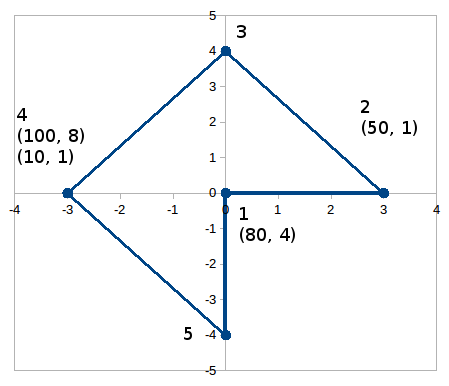
\includegraphics[width=0.6\linewidth]{figuras/pmv/mapaItens}
    \caption{Mapa de cidades e seus itens}
    \label{fig:mapaItens}
\end{figure}

Tomemos como exemplo a seguinte rota sem nenhum item coletado $x = \{ 1, 2, 3, 4, 5 \}$ logo $y = \{ 0, 0, 0, 0 \}$.
Para essa solução teremos o valor de função objetivo igual a -55,00.

Consideremos a gora a mesma rota coletando o item de maior lucro associado, então temos a rota $x = \{ 1, 2, 3, 4, 5 \}$, e a mochila $y = \{ 0, 0, 1, 0 \}$.
Agora teremos uma solução de valor -157,00.

Considerando ainda a mesma rota mas com dois itens coletados, temos a rota $x = \{ 1, 2, 3, 4, 5 \}$, e a mochila $y = \{ 0, 1, 0, 1 \}$.
Neste caso temos um valor de função objetivo igual a -4.70.


Nas Figuras~\ref{fig:pmvExemplo}, \ref{fig:pmvExemploAlterandoItens} e \ref{fig:pmvExemploAlterandoInicio} podemos ver a representação de soluções diferentes para a mesma instância de um PMV.
Cada apontador indica uma cidade sem itens a serem coletados, os presentes indicam itens a serem coletados com dois números associados ($p_i / w_i$, sendo $w_i$ e $p_i$ o peso e o lucro associados ao item $i$ respectivamente).
O stickman representa o início da rota, $W$ representa a capacidade de carga do veículo e $R$ a taxa de aluguel cobrada por unidade de tempo de uso do mesmo.

\begin{figure}[htpb]
    \centering
    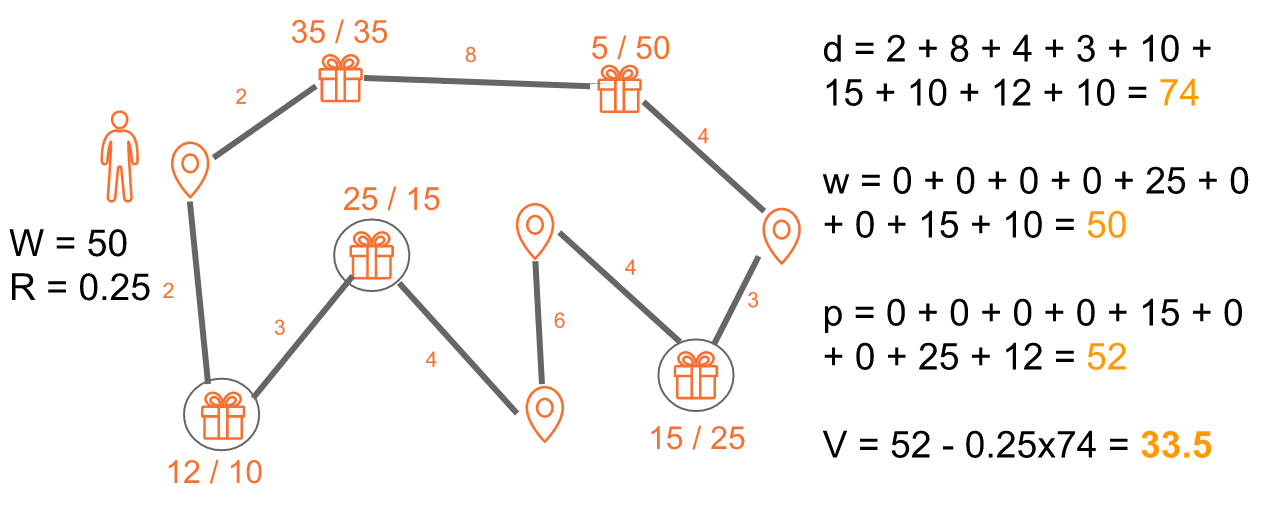
\includegraphics[width=0.8\linewidth]{figuras/pmv/example01.png}
    \caption{Exemplo de representação visual do PMV}
    \label{fig:pmvExemplo}
\end{figure}

Pelo primeiro exemplo, na Figura~\ref{fig:pmvExemplo}, vemos que são coletados 3 itens de valores 15, 25 e 12; e pesos de valor 25, 15, 10.
Desta forma temos um percurso total de distância 74, peso final do caminhão de 50, valor dos itens de 52.
Todos estes fatores aplicados à fórmula da função objetivo conferem um valor de solução de 33,5.

\begin{figure}[htpb]
    \centering
    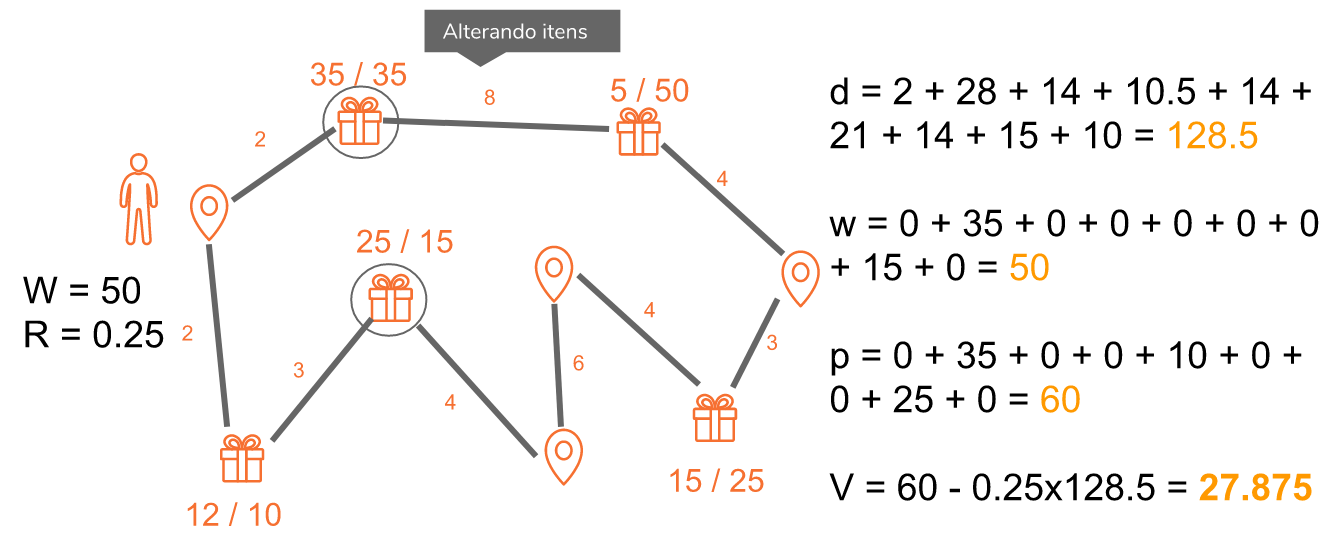
\includegraphics[width=0.8\linewidth]{figuras/pmv/example02.png}
    \caption{Mesmo conjunto de cidades e itens, alterando os itens coletados.}
    \label{fig:pmvExemploAlterandoItens}
\end{figure}

Mantendo a mesma rota do exemplo da Figura~\ref{fig:pmvExemplo} apenas alterando os itens coletados temos o exemplo da Figura~\ref{fig:pmvExemploAlterandoItens} que coleta apenas 2 itens de valores 35 e 25; além de pesos 35 e 15.
Neste caso se tem o mesmo peso final de 50 e um maior valor dos itens 60, contra 50 da solução anterior, porém coletar o item mais valioso e pesado logo no começo da rota prejudica todo o percurso fazendo com que sejam gastas muito mais unidades de tempo para percorrer todo o percurso, sendo um total de 128,5.
Logo temos um valor final de função objetivo de 27,875 que é menor que o anterior mesmo tendo coletado itens mais valiosos, isto ocorre porque apesar dos itens mais valiosos o custo pra coletá-los foi maior.

\begin{figure}[htpb]
    \centering
    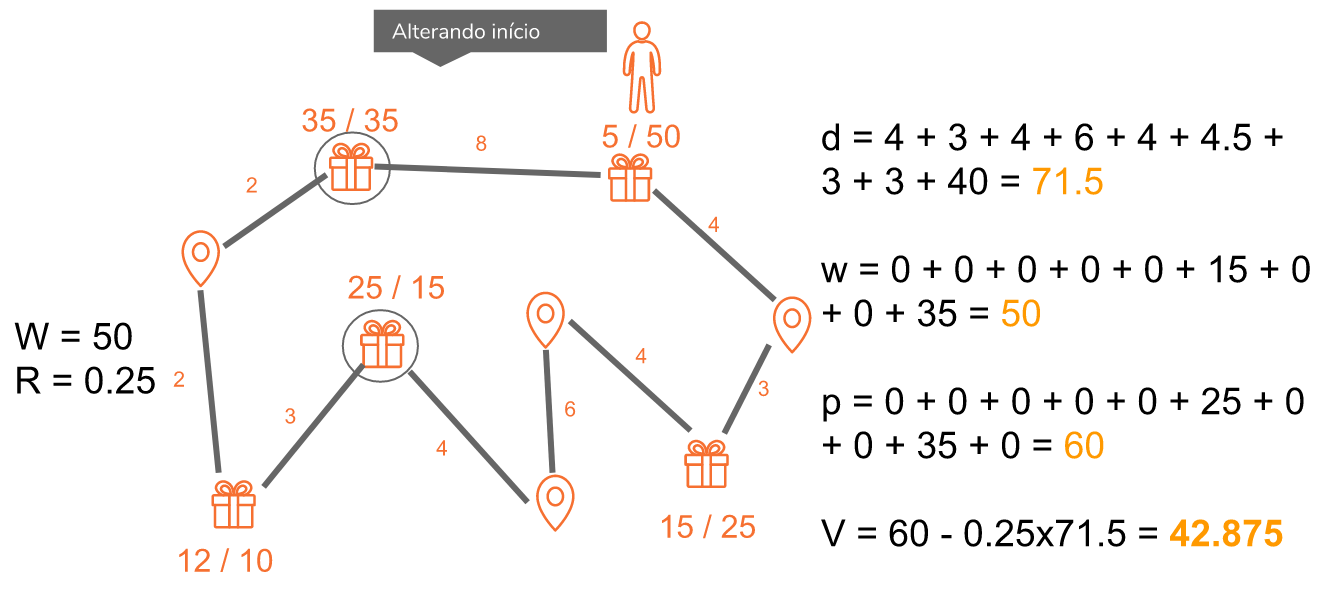
\includegraphics[width=0.8\linewidth]{figuras/pmv/example03.png}
    \caption{Mesmo conjunto de cidades e itens, alterando inicio da rota.}
    \label{fig:pmvExemploAlterandoInicio}
\end{figure}

No caso da Figura~\ref{fig:pmvExemploAlterandoInicio} foram mantidos os itens da Figura~\ref{fig:pmvExemploAlterandoItens} contudo foi trocada a cidade inicial do problema de forma que o veículo não precise transportar o item mais pesado por um período muito longo diminuindo assim o custo da rota para 71,5.
Não tendo alterado o os itens coletados o peso final e valor dos itens também se mantem constante, desta forma o novo valor de função objetivo é de 42,875 superando os valores encontrados nas duas soluções anteriores.

Mais alguns exemplos ilustrando o problema podem ser encontrados em \cite{Bonyadi:2013, Oliveira:2015}.


\section{Problema da Mínima Latência}\label{sec:mlp}

O Problema da Mínima Latência (PML) é um problema de otimização, sendo uma variante do PCV no qual o objetivo é minimizar o tempo de chegada (ou latência) aos vértices, e não a distância ou tempo da rota como no problema original.
O PML pode ser definido como um grafo direcionado $G=(V,E)$, onde $V=\{0,1,\dots,n\}$ é um conjunto de vértices e $E = \{(i, j) : i, j \in V, i \ne j \}$ um conjunto de arestas que conectam os vértices.
Para cada arco $(i,j)$ existe um tempo de viagem associado igual a $t(i,j)$. O vértice 0 representa o ponto de saída (depósito) e os demais os clientes a serem visitados.
O tempo de chegada (ou latência) a um cliente $i \in V$, é denotado por $l(i)$, o qual é definido pelo tempo de viagem do depósito até o vértice $i$.

\begin{figure}[htpb]
    \centering
    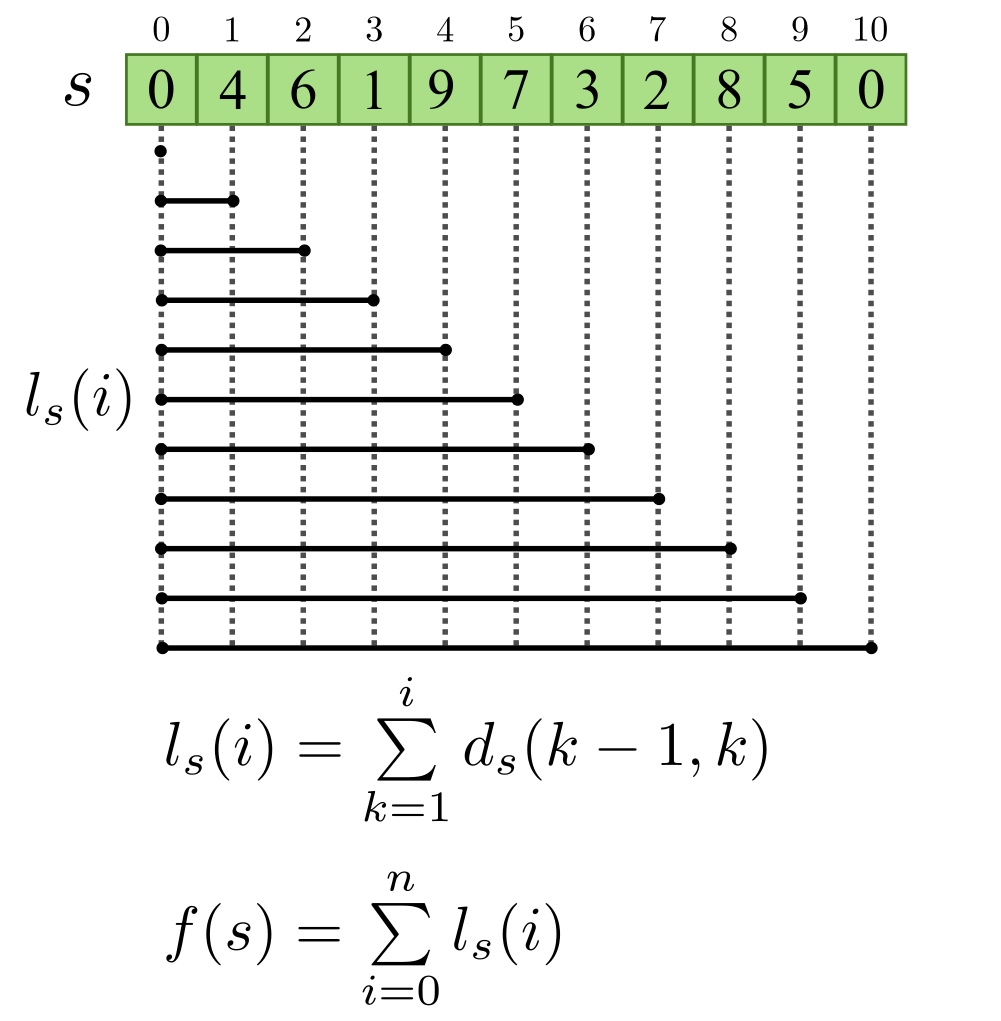
\includegraphics[width=0.6\linewidth]{figuras/pml/mlp}
    \caption{Exemplo de solução com as latências de cada cidade e cálculo da função objetivo}
    \label{fig:pmlDiagramaFormulas}
\end{figure}

O objetivo do PML é, iniciando do depósito, determinar o ciclo Hamiltoniano $s$ que minimize a latência expressa por $L(s)=\sum_{i=0}^{n} l(i)$ como pode ser visto na Figura~\ref{fig:pmlDiagramaFormulas}.
Assim sendo, uma solução viável do PML consiste numa permutação de $n$ clientes determinando a ordem de visita dos mesmos. Tomemos o exemplo a seguir, se $n=9$,  $s=[0,8,3,7,1,4,2,5,6,0]$ é uma solução viável para o PML (de fato, qualquer permutação $1..8$ começando e terminando no vértice zero é uma solução viável).

Apesar da formulação simples e de sua grande aplicação na otimização de latência em redes, o PML é um problema complexo, sendo provado que o PML é NP-Difícil~\cite{silva2012}. A despeito da semelhança na formulação do PML com a do Problema do Caixeiro Viajente (PCV) a sua função objetivo é mais complexa de ser calculada que a do PCV.
No PML, pequenas alterações no vetor solução podem levar a grandes alterações no resultado final da solução e a natureza não local da função objetivo faz com que uma simples inserção afete todas as latências subsequentes.
Na literatura, o PML também é conhecido Problema do Caixeiro Viajante Cumulativo \cite{bianco1993}, Problema do Entregador \cite{mladenovic2013} e Problema do Reparador Viajante. \cite{tsitsiklis1992}.

Em trabalhos recentes, um procedimento de busca local baseado em \emph{Graphics Processing Unit} (\emph{GPU}) e computação \emph{multi-core} foi proposto para o PML~\cite{wamca2016}.
A ideia foi chamada \emph{Distributed Variable Neighborhood Descent} (\emph{DVND}), tentando explorar diferentes estratégias de vizinhança simultaneamente para uma solução de entrada.

Em otimização, uma vizinhança é definida como um conjunto de operações chamados "movimentos", que são capazes de realizar pequenas alterações na solução de entrada.
Estas alterações podem ser, por exemplo, trocar dois elemento na permutação inicial, gerando dessa forma $\mathcal{O}(N^2)$ diferentes soluções (para o caso de uma permutação de tamanho $N$). Existe na literatura muitas dessas vizinhanças (como 2-Opt, OrOpt-1, OrOpt-2, Swap, ..., etc), conquanto por limitações computacionais estes são sempre explorados de forma sequencial, chamados de \emph{Variable Neighborhood Descent} (\emph{VND}).
Com o objetivo de encontrar um ótimo local para o PML, a ideia principal do DVND é usar GPU para obter operações de grão fino (que em geral são rápidas) e explorar toda a vizinhança $\mathcal{O}(N^2)$ mais rápido que em CPU (como explicado em~\cite{wamca2016}) e combinar as respostas das buscas, escolhendo a nova melhor solução.

\subsection{Exemplo}

% \begin{figure}[htpb]
%     \centering
%     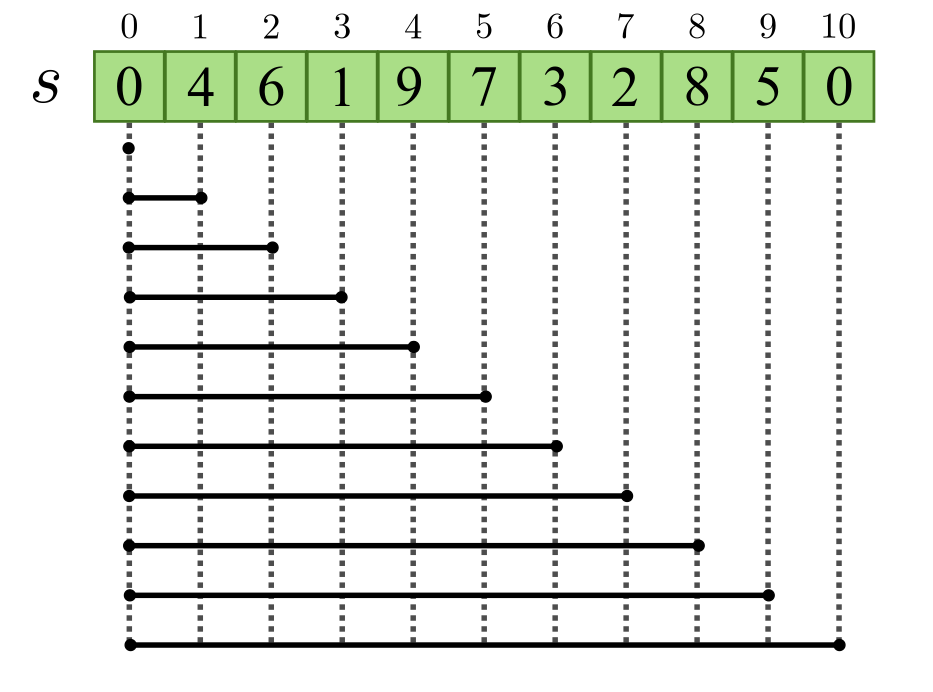
\includegraphics[width=0.6\linewidth]{figuras/pml/mlp-clean}
%     \caption{Exemplo de solução com as latências de cada cidade}
%     \label{fig:pml}
% \end{figure}

Pelo exemplo na Figura~\ref{fig:pmlDiagramaFormulas} podemos ver que o valor da latência $L(s)$ será dado palos somatórios das latências de todas as cidades, sendo $d_s^{i, j}$ a distância da cidade $i$ para a cidade $j$ na solução $s$, então temos:
$$ L(s) = \sum_{i=0}^n{l_s(i)} $$
$$ L(s) = l_s(0) + l_s(1) + l_s(2) + l_s(3) + l_s(4) + l_s(5) + l_s(6) + l_s(7) + l_s(8) + l_s(9) $$
$$ L(s) = 10d_s^{0, 4} + 9d_s^{4, 6} + 8d_s^{6, 1} + 7d_s^{1, 9} + 6d_s^{9, 7} + 5d_s^{7, 3} + 4d_s^{3, 2} + 3d_s^{2, 8} + 2d_s^{8, 5} + d_s^{5, 0}$$

